\chapter{Fonctions affines}

\section{Introduction et exemple concret}

\begin{ex}[Situation des compagnies de bus]
	Pour un voyage scolaire, une classe de Première STMG compare les tarifs de deux compagnies de transport :
	\begin{itemize}
		\item \textbf{Compagnie A :} applique un forfait fixe de $15\eur{}$ auquel s'ajoute $2\eur{}$ par kilomètre parcouru.
		\item \textbf{Compagnie B :} ne facture pas de forfait fixe, mais facture $3,50\eur{}$ par kilomètre parcouru.
	\end{itemize}

	Si on note $x$ le nombre de kilomètres parcourus :
	\begin{itemize}
		\item Le prix payé avec la compagnie A est : $f(x) = 2x + 15$.
		\item Le prix payé avec la compagnie B est : $g(x) = 3,50x$.
	\end{itemize}

	Les fonctions $f$ et $g$ ainsi définies sont des \textbf{fonctions affines}.
\end{ex}

\section{Définitions et vocabulaire}

\subsection{Fonction affine}

\begin{defn}[Fonction affine]
	Soit $m$ et $p$ deux nombres réels donnés.

	Une \textbf{fonction affine} $f$ est une fonction définie sur $\R$ par l'expression :
	\[
		f(x) = mx + p
	\]

	\begin{itemize}
		\item Le nombre $m$ est appelé le \textbf{coefficient directeur}.
		\item Le nombre $p$ est appelé l'\textbf{ordonnée à l'origine}.
	\end{itemize}
\end{defn}

\begin{rem}[Cas particuliers]
	\nline
	\begin{itemize}
		\item Si $p = 0$, alors $f(x) = mx$ : on dit que $f$ est une \textbf{fonction linéaire} (situation de proportionnalité).
		\item Si $m = 0$, alors $f(x) = p$ : on dit que $f$ est une \textbf{fonction constante}.
	\end{itemize}
\end{rem}

\begin{ex}
	\nline
	\begin{itemize}
		\item $f(x) = 3x - 5$ est une fonction affine avec $m = 3$ et $p = -5$.
		\item $g(x) = -2x + 7$ est une fonction affine avec $m = -2$ et $p = 7$.
		\item $h(x) = 4x$ est une fonction affine (et linéaire) avec $m = 4$ et $p = 0$.
		\item $k(x) = 6$ est une fonction affine (et constante) avec $m = 0$ et $p = 6$.
	\end{itemize}
\end{ex}

\subsection{Calcul d'une image et d'un antécédent}

\begin{methode}[Calculer une image ou un antécédent]
	Soit la fonction affine $f(x) = 2x + 15$ (tarifs de la compagnie A).
	\begin{enumerate}
		\item Calculer le prix pour un trajet de $40\text{ km}$ (image de $40$).
		\item Déterminer le nombre de kilomètres parcourus pour un montant de $55\eur{}$ (antécédent de $55$).
	\end{enumerate}

	\begin{correction}
		\nline
		\begin{enumerate}
			\item On calcule $f(40)$ :
			      \[
				      f(40) = 2 \times 40 + 15 = 80 + 15 = 95
			      \]
			      Le prix pour $40\text{ km}$ est de $95\eur{}$.

			\item On cherche $x$ tel que $f(x) = 55$ :
			      \[
				      2x + 15 = 55 \eqv 2x = 40 \eqv x = 20
			      \]
			      Pour un montant de $55\eur{}$, la distance parcourue est de $20\text{ km}$.
		\end{enumerate}
	\end{correction}
\end{methode}

\section{Représentation graphique}

\begin{prop}[Représentation graphique d'une fonction affine]
	Dans un repère du plan, la représentation graphique d'une fonction affine $f(x) = mx + p$ est une \textbf{droite}.
	\begin{itemize}
		\item $p$ est l'ordonnée du point d'intersection de la droite avec l'axe vertical $(0\,;\,p)$.
		\item Le coefficient directeur $m$ caractérise la pente de la droite.
	\end{itemize}
\end{prop}

% TODO illustration à revoir
\begin{center}
	\begin{tikzpicture}[>=Stealth]
		\draw[->] (-1,0) -- (5,0) node[above] {$x$};
		\draw[->] (0,-1) -- (0,4) node[right] {$y$};
		\draw[ultra thick, blue, domain=-1:5] plot ( \x , 0.5*\x+1 );
		% \draw[thick, blue] (-0.5,0.5) -- (4.5,4.5) node[right] {$y = mx + p$};
		\fill (0,1) circle (3pt) node[above left] {$p$};
		\draw[dashed] (1,1.5) -- (3,1.5) -- (3,2.5);
		\node at (2,1.2) {$1$};
		\node at (3.4,2) {$m$};
	\end{tikzpicture}
\end{center}
\begin{methode}[Tracer la droite représentant une fonction affine]
	Pour tracer la droite représentant la fonction $f(x) = 2x + 15$ sur l'intervalle $[0\,;\,30]$ :
	\begin{enumerate}
		\item On calcule les coordonnées de deux points (par exemple pour $x = 0$ et $x = 20$) :
		      \begin{itemize}
			      \item Si $x = 0$, $f(0) = 2(0) + 15 = 15$ (Point $A(0\,;\,15)$).
			      \item Si $x = 20$, $f(20) = 2(20) + 15 = 55$ (Point $B(20\,;\,55)$).
		      \end{itemize}
		\item On place ces deux points dans le repère et l'on trace la droite passant par $A$ et $B$.
	\end{enumerate}
\end{methode}

\section{Sens de variation}

\begin{prop}[Sens de variation d'une fonction affine]
	Soit $f(x) = mx + p$ une fonction affine sur $\R$. Le sens de variation de $f$ dépend du signe de son coefficient directeur $m$ :
	\begin{itemize}
		\item Si $m > 0$, la fonction $f$ est \textbf{croissante} sur $\R$.
		\item Si $m < 0$, la fonction $f$ est \textbf{décroissante} sur $\R$.
		\item Si $m = 0$, la fonction $f$ est \textbf{constante} sur $\R$.
	\end{itemize}
\end{prop}

\begin{ex}
	\nline
	\begin{itemize}
		\item Pour la fonction $f(x) = 2x + 15$ (compagnie A), on a $m = 2 > 0$ : la fonction est \textbf{croissante}. Plus on roule, plus le prix augmente.
		\item Pour la fonction $g(x) = -1,5x + 50$, on a $m = -1,5 < 0$ : la fonction est \textbf{décroissante}.
	\end{itemize}
\end{ex}

\begin{prop}[Tableau de variation]
	Voici l'allure générale du tableau de variation d'une fonction affine selon le signe de $m$ :

	\begin{center}
		\begin{tabular}{cc}
			\textbf{Si $m > 0$ (Croissante)} & \textbf{Si $m < 0$ (Décroissante)} \\
			\begin{tikzpicture}
				\tkzTabInit[lgt=1,espcl=2.5]{$x$ / 1, $f$ / 2}{$-\infty$, $+\infty$}
				\tkzTabVar{-/ , +/}
			\end{tikzpicture}
			                                 &
			\begin{tikzpicture}
				\tkzTabInit[lgt=1,espcl=2.5]{$x$ / 1, $f$ / 2}{$-\infty$, $+\infty$}
				\tkzTabVar{+/ , -/}
			\end{tikzpicture}
		\end{tabular}
	\end{center}
\end{prop}

\section{Étude du signe}

\begin{prop}[Signe d'une expression affine]
	Soit $f(x) = mx + p$ avec $m \neq 0$.
	L'expression s'annule pour la valeur (appelée racine) :
	\[
		x = -\dfrac{p}{m}
	\]
	Le signe de $mx + p$ est donné par la règle suivante : \textbf{le signe de $m$ après la racine, et le signe contraires de $m$ avant la racine}.
\end{prop}

\begin{methode}[Établir le tableau de signes]
	Pour étudier le signe de $f(x) = 2x - 6$ :
	\begin{enumerate}
		\item On résout l'équation $2x - 6 = 0 \eqv 2x = 6 \eqv x = 3$.
		\item Le coefficient directeur est $m = 2 > 0$.
	\end{enumerate}
	Le tableau de signes est donc :
	\begin{center}
		\begin{tikzpicture}
			\tkzTabInit[lgt=2,espcl=3]{$x$ / 1, $2x - 6$ / 1}{$-\infty$, $3$, $+\infty$}
			\tkzTabLine{,-,0,+,}
		\end{tikzpicture}
	\end{center}
\end{methode}

\section{Résolution d'équations et d'inéquations}

\subsection{Résolution d'une équation $f(x) = g(x)$}

\begin{methode}[Résoudre $f(x) = g(x)$]
	Revenons à nos deux compagnies de bus avec :

	\begin{itemize}
		\item $f(x) = 2x + 15$ (Compagnie A)
		\item $g(x) = 3,50x$ (Compagnie B)
	\end{itemize}

	À partir de combien de kilomètres les deux compagnies coûtent-elles exactement le même prix ?

	\begin{correction}
		On résout l'équation $f(x) = g(x)$ :
		\[
			2x + 15 = 3,50x
		\]
		\[
			15 = 3,50x - 2x
		\]
		\[
			15 = 1,50x
		\]
		\[
			x = \dfrac{15}{1,50} = 10
		\]
		Pour un trajet de $10\text{ km}$, les deux compagnies coûtent le même prix ($35\eur{}$).
	\end{correction}
\end{methode}

\subsection{Résolution d'une inéquation $f(x) < g(x)$}

\begin{methode}[Résoudre une inéquation entre fonctions affines]
	En reprenant les compagnies A et B, à partir de quelle distance la compagnie A devient-elle plus avantageuse que la compagnie B ?

	\begin{correction}
		On cherche à résoudre l'inéquation $f(x) < g(x)$ :
		\[
			2x + 15 < 3,50x
		\]
		\[
			15 < 3,50x - 2x
		\]
		\[
			15 < 1,50x
		\]
		\[
			x > \dfrac{15}{1,50} \eqv x > 10
		\]
		La compagnie A est plus avantageuse pour un nombre de kilomètres \textbf{strictement supérieur à $10\text{ km}$}.
	\end{correction}
\end{methode}
